\documentclass[10pt]{article}
\usepackage{icmlko}

\icmlmeta{IP 파운데이션 월드모델}{334}{그림자를 다 지웠는데 축이 안 살아났다}{앨범 메타까지 긁어 풀 그림자가 0 이 됐다 --- 그런데 뺐던 축 둘을 되살리면 1/12 만 이긴다}

\begin{document}

\twocolumn[
\icmlheader

\begin{abstract}
노트 333이 남긴 마지막 그림자 --- 앨범 메타 --- 를 다 긁었다(81$\to$175건,
버전 확보 70$\to$151). \textbf{이제 셋 다 깨끗하다}: 위키 $+$0.15 · 검색
$-$0.03 · 앨범 메타 $-$0.02, \texttt{poolshadow} 판정 \textbf{``풀 그림자
--- 없음''}.

\textbf{그래서 노트 326이 뺐던 축 둘을 되살렸다.} 그때 뺀 이유는 축이
나빠서가 아니라 \emph{그 표시자가 한터 여부와 99.4\% 같았기} 때문이고,
좁은 판에서는 $+$0.039 를 벌고 있었다. \textbf{미리 적었다} --- ``그림자를
지웠으니 $+$0.039 근처를 기대한다.''

\textbf{틀렸다.} 되살리면 아이돌이 0.5115 $\to$ \textbf{0.2738} 로 내려간다.
짝지어(학습 재추출 열둘) 재면 \textbf{$-$0.0708(SD 0.0642 · 양수 1/12)}
이고 판도 $-$0.0035 다. \textbf{그림자를 지워도 축은 안 살아난다.}

\textbf{그래서 배포할 것은 ``뺀 채''다.} 행을 넓히고 위키 · 검색을
되살리되 앨범 메타 파생 축 둘은 계속 뺀다 --- 현행 판 대비 아이돌
\textbf{$+$0.2474(SD 0.1254 · 12/12)} · 판 $+$0.0049(SD 0.0075, 미결정 폭
0.010 안). \textbf{같은 유보 25행에서 0.2385 $\to$ 0.5115 다.}

\textbf{왜 안 살아났나는 아직 모른다.} 갈래 셋을 적어 둔다 --- ① 새로 긁은
94건의 매칭 품질이 낮다(그룹명$+$앨범명 둘 다 걸려야 채택하는데 덜 유명한
그룹은 상품 페이지가 거칠다) ② 두 축이 유보 25행에 열 넷을 더한다(값 둘 ·
표시자 둘) ③ 축 자체가 원래 약했고 좁은 판의 $+$0.039 가 잡음이었다.
\end{abstract}
]

\section{그림자가 0 이 됐다}

\begin{center}\small
\begin{tabular}{lrrl}
\hline
재료 & 전 & 후 & 판정 \\
\hline
위키 & $+$0.99 & $+$0.15 & 괜찮다 \\
검색 & $+$0.18 & $-$0.03 & 괜찮다 \\
앨범 메타 & $+$1.00 & \textbf{$-$0.02} & 괜찮다 \\
\hline
\end{tabular}
\end{center}

앨범 메타는 한터 85\% 대 추가 \textbf{87\%} --- 추가 쪽이 오히려 높다.
수집기 셋을 다 고치고 다 돌린 결과다(노트 332 · 333 · 334).

\begin{figure*}[t]
\centering
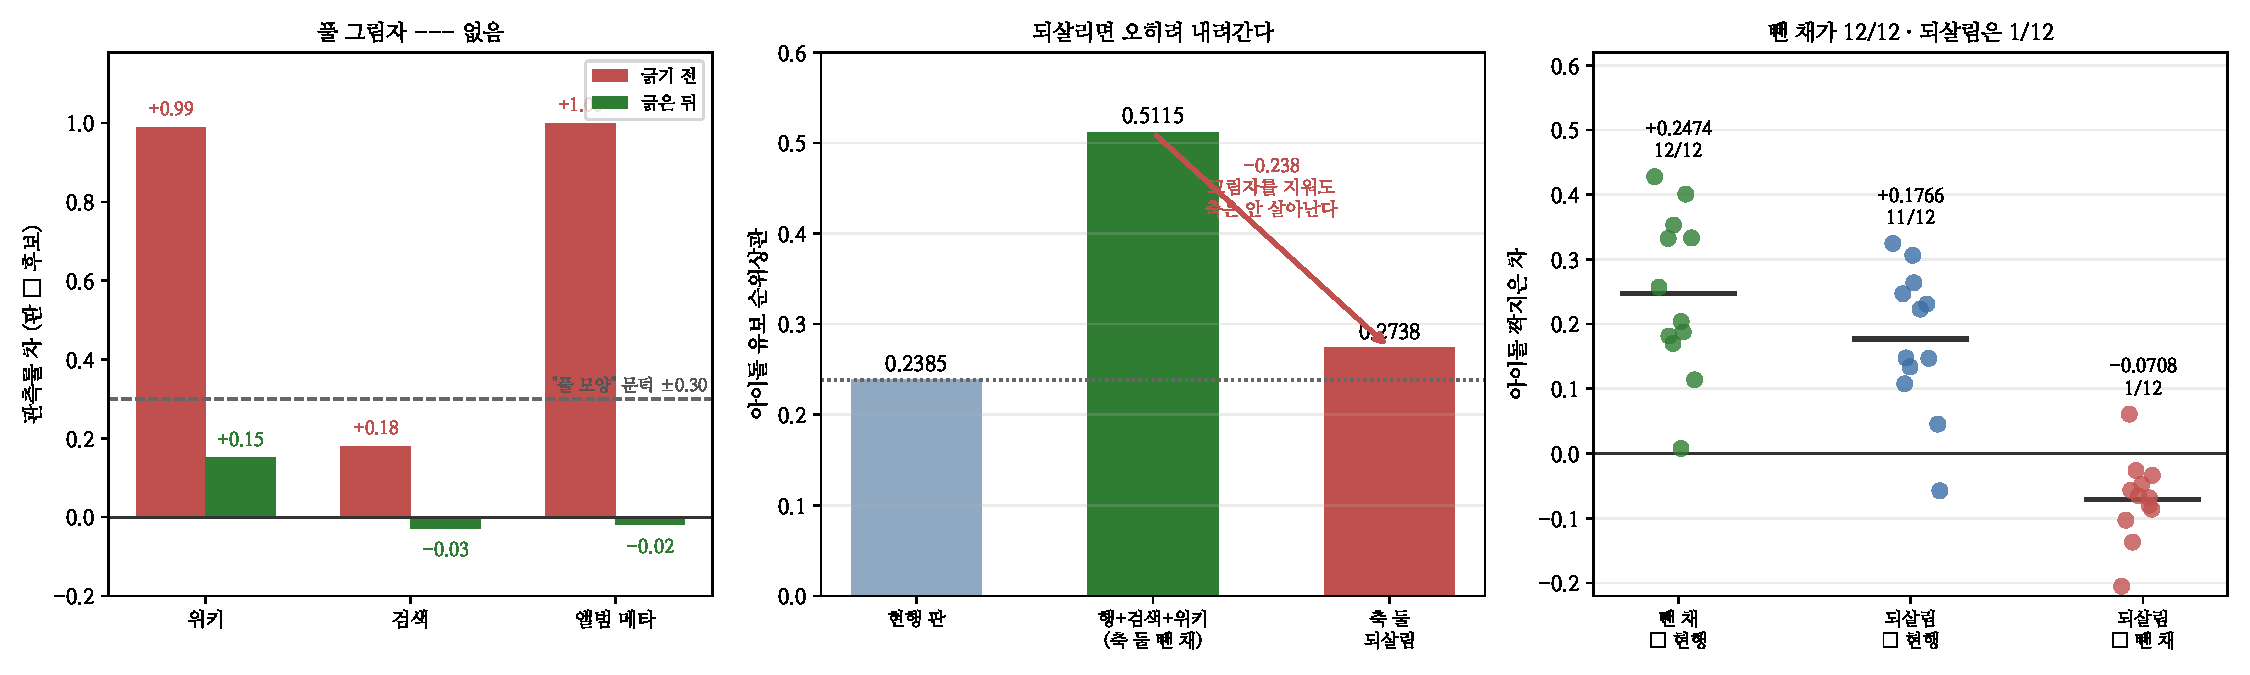
\includegraphics[width=\textwidth]{figs/lifted.pdf}
\caption{왼쪽 --- 세 재료의 그림자. 가운데 --- 아이돌 사다리.
오른쪽 --- 짝지은 차.}
\end{figure*}

\section{그런데 축이 안 살아났다}

\begin{center}\footnotesize
\begin{tabular}{lrr}
\hline
팔 & 판 & 아이돌 \\
\hline
현행 \texttt{trendcalwikitag} & 0.4725 & 0.2385 \\
\textbf{행$+$검색$+$위키(축 둘 뺀 채)} & \textbf{0.4763} & \textbf{0.5115} \\
\quad $+$축 둘 되살림 & 0.4618 & 0.2738 \\
\hline
\end{tabular}
\end{center}

\begin{center}\footnotesize
\begin{tabular}{lrrr}
\hline
짝지은 차 & 아이돌 & SD & 양수 \\
\hline
뺀 채 $-$ 현행 & \textbf{$+$0.2474} & 0.1254 & \textbf{12/12} \\
되살림 $-$ 현행 & $+$0.1766 & 0.1115 & 11/12 \\
\textbf{되살림 $-$ 뺀 채} & \textbf{$-$0.0708} & 0.0642 & \textbf{1/12} \\
\hline
판(뺀 채 $-$ 현행) & $+$0.0049 & 0.0075 & \\
판(되살림 $-$ 뺀 채) & $-$0.0035 & 0.0040 & \\
\hline
\end{tabular}
\end{center}

\textbf{미리 적은 기대가 틀렸다.} 노트 326에서 그 둘은 좁은 판(79행)에서
$+$0.0393 을 벌고 넓힌 판에서 $-$0.1246 을 잃었고, 나는 그 손해를
\emph{전부} 그림자 탓으로 읽었다. 그림자를 없앤 지금도 $-$0.0708 이다 ---
\textbf{손해의 절반은 그림자가 아니었다.}

\section{배포할 것}

\begin{center}\small
\begin{tabular}{ll}
\hline
행 & 한터 79 $+$ 추가 68 $=$ 147 (유보 25 그대로) \\
위키 & 되살림 (173건 다 긁음) \\
검색 & 되살림 (44 $\to$ 169건) \\
앨범 축 둘 & \textbf{계속 뺀다} \\
\hline
판 & $+$0.0049 (미결정 폭 0.010 안) \\
아이돌 & \textbf{$+$0.2474 · 12/12} \\
\hline
\end{tabular}
\end{center}

\textbf{배포 규칙 ①②를 통과한다} --- 판이 폭 안이고 어느 도메인도
문턱 밖으로 안 내려간다. 그리고 \textbf{자료 결정이지 점수로 고른 것이
아니다}(노트 82 · 90) --- 필터를 뗀 것과 수집기를 끝까지 돌린 것뿐이다.

\section{왜 안 살아났나}

\begin{center}\footnotesize
\begin{tabular}{ll}
\hline
갈래 & 어떻게 가르나 \\
\hline
① 새 94건 매칭이 거칠다 & \texttt{n\_hits} 로 나눠 재라 \\
② 열이 25행에 많다 & 값만/표시자만으로 갈라라 \\
③ 원래 약했다 & 좁은 판 $+$0.039 를 다시 재라 \\
\hline
\end{tabular}
\end{center}

\section{남은 것}
\begin{center}\footnotesize
\begin{tabular}{ll}
\hline
갈래 & 왜 \\
\hline
\textbf{만화 검색 5\%} & 1,473 긁어 상태 73 \\
축 둘이 왜 해로운가 & 갈래 셋 \\
아이돌 넓힘을 승격 & 판 폭 안 · 도메인 두 배 \\
세계애니 검색 1,311 & 만화처럼 비어 있을까 \\
\hline
\end{tabular}
\end{center}

\paragraph{덤 --- 만화 검색을 긁어 봤다} 노트 333이 ``검색이 0\% 인 것은
그림자가 아니라 게으름''이라 했고, 그 말대로 만화 1,473건을 다 돌렸다.
\textbf{상태가 나온 것은 73건(5\%)이다.} 게임 영문 질의가 67\% 였던 것과
전혀 다르다 --- 데이터랩에 그 제목들의 검색량이 거의 없다.
\textbf{노트 149가 위키 축을 만든 판단은 옳았다.} 다만 그때 적은 이유
(``제목이 한국어가 아니다'')는 절반만 맞았다 --- 돌려 보니 질의는 되고
\emph{답이 비어 있다}. \textbf{안 해 봐서 몰랐던 것과 해 보니 없는 것은
다르고, 오늘 그 둘이 갈렸다.}

\paragraph{규약} \textbf{원인을 지웠다고 결과가 돌아오지는 않는다.} 노트
326이 축 둘의 손해를 그림자로 설명했고 그 설명은 \emph{맞았다} --- 표시자가
한터 여부와 99.4\% 같았으니까. 그런데 그림자를 지우고 나니 손해가 반만
사라졌다. \textbf{설명이 맞다는 것과 그것이 전부라는 것은 다르다.}
그리고 이 판에서 그 차이를 아는 유일한 방법은 \textbf{고친 뒤에 다시
재는 것}이었다 --- 고치기 전에는 두 원인이 겹쳐 있어 못 갈랐다.

\end{document}
